
\section{Challenges In FaaS Load-balancing}
\label{sec:challenges}
Load balancing in FaaS clusters represents a unique set of challenges which we describe in this section.
We motivate our observations using the Azure function trace~\cite{shahrad_serverless_2020}, as well as empirical performance measurements conducted using OpenWhisk.  

% \subsection{Importance of locality}

% % Function locality is important, but non-uniform. % Are we using this non-uniformity anywhere?
% % The cold/warm times can vary significantly.
% % Show this using the real FaaSBench results. 

% Both the user and provider place importance on locality in FaaS.
% Cold-start functions have significant overhead, costing user time and the provider CPU cycles.
% Table~\ref{tab:func-times} lists a variety of functions we have converted from FunctionBench \cite{kim_functionbench_2019}
% Latencies of cold start functions can be similar to the warm start latency, but are more often several times higher.
% Avoiding these cold starts as much as possible is vital to effective FaaS balancing.
%\vspace*{-0.2cm}
\subsection{Function Heterogeneity and Skew}


\begin{figure}
  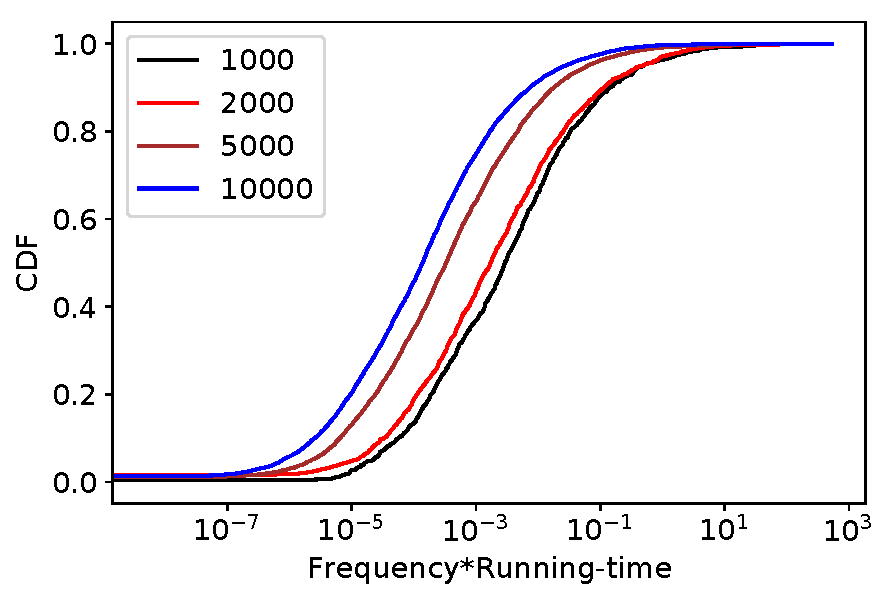
\includegraphics[width=0.35\textwidth]{../figs/freqs-all.pdf}
 %   \vspace*{-0.2cm}
  \caption{Function load is very heavy tailed (note the log X axis). Each line represents a different random subset and associated subset size from the Azure function trace. }
  \label{fig:freqs}
  %  \vspace*{-0.2cm}
\end{figure}

For locality-sensitive load-balancing techniques to be effective, it is important for each function to impose roughly similar load on the system. 
However, functions vary widely in their frequency of invocation as well as their running time. 
The running-time heterogeneity of functions can be seen in Table~\ref{tab:func-times}, which shows that the times can range from 100ms to almost one minute.
Thus, the computing requirements (in terms of running time) of functions are highly heterogeneous. 

The popularities of the functions (i.e., their invocation frequency) is also highly skewed. 
Figure~\ref{fig:freqs} shows the distribution of the frequency $\times$ running-time, for four randomly sampled subsets of functions from the Azure trace. 
This metric is effectively the ``induced-load'' of a function. 
We see that the functions are extremely heavy tailed in their induced-load: the ``heavy'' top 20\% functions consume 2 orders of magnitude more resources than the average. 
Thus, with classic consistent hashing the servers handling the heavy functions will be extremely overloaded, which will contribute to severe function slow-down due to resource contention on the servers. 

%\vspace*{-0.2cm}
\subsection{Bursty Invocations}

The second challenge is that the function arrivals can be very bursty and can vary widely by function. 
Figure~\ref{fig:iats} shows the inter-arrival-time (IAT) distribution computed from the Azure functions dataset. 
We see the average IAT of functions varies widely (the ``All'' line in the figure): by more than seven orders of magnitude.

Importantly, the IAT of the popular functions (ordered by number of invocations) can be significantly lower and different. For instance, for the top 10\% of the popular functions, their $90^{th}$ percentile IAT is less than 1 second. In contrast, the $90^{th}$ percentile IAT for all functions is 2,000 seconds.
%
This heavily skewed workload also has significant ramifications for Load Balancing, since we must be able to handle highly bursty functions, as well as the long tail of infrequently invoked functions.
This fairness in function handling is thus an important challenge in FaaS load balancing. 


\begin{figure}
  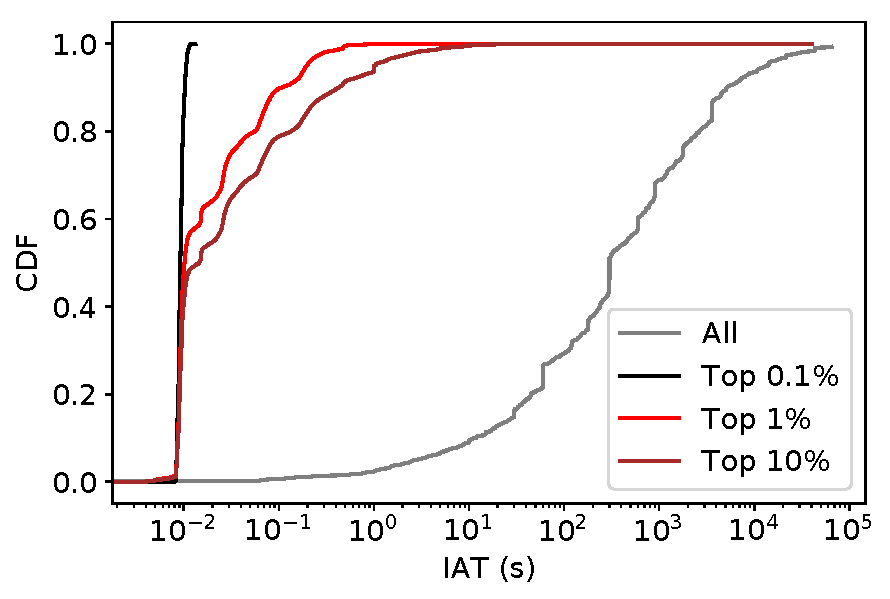
\includegraphics[width=0.35\textwidth]{../figs/iats-all.pdf}
%    \vspace*{-0.2cm}
  \caption{Inter arrival times of popular functions can be extremely low, and show a very wide variance (note the log-scale of the X axis).}
  \label{fig:iats}
 % \vspace*{-0.2cm}
\end{figure}

%\vspace*{-0.2cm}
\subsection{Function Performance and Server Load}
\label{subsec:function-perf}
% Here or next section?

Our goal is to minimize the total end-to-end function execution latency. 
Unlike classic data-oriented load-balancing, function execution latency can be highly sensitive to the server load.
That is, running on an overloaded server (even if it is a warm-start), can result in significant latency increase and performance degradation.

Function performance can be affected by many factors such as the number of concurrently running functions, the CPU utilization, the load-average, interference due to other co-located functions, etc.
The slowdown in a processor-sharing system due to system load has been well modeled.
Queuing theory approaches for G/G/PS systems approximate the running time of a task to be proportional to $1/1-\rho$, where $\rho$ is the system utilization/load.

However, function heterogeneity and their execution characteristics presents many challenges in modeling and understanding their performance.
We have found that the container initialization and other OpenWhisk overheads, \emph{even for warm starts}, can be a significant source of latency, slowdown, and jitter. 

% \begin{table}
%   \begin{tabular}{ c c c c }
% \hline
%   Application & Min Time (s) & Mean Time (s) & $99^{th}$ Pctl (s) \\ 
% \hline
%   Web-serving & 0.015 & 0.408 & 1.049 \\  
%   ML Inference (CNN) & 0.166 & 0.405 & 2.299 \\
%   Disk-bench (dd) & 0.016 & 1.123 & 2.534 \\  
%   % float & 0.014 & 0.148 & 1.026 \\  
%   % gzip & 0.014 & 0.157 & 1.065 \\  
%   % image & 0.014 & 0.213 & 2.697 \\  
%   Matrix Multiply & 0.013 & 0.159 & 1.054 \\  
%   Sklearn Regression & 0.15 & 2.32 & 11.06 \\  
%   AES Encryption & 0.015 & 0.171 & 1.221 \\  
%   Video Encoding & 0.15 & 1.138 & 9.96 \\  
%   JSON Parsing & 0.015 & 0.159 & 1.012 \\
% \hline
% \end{tabular}
% \caption{The system overhead on warm invocations for the functions from Table~\ref{tab:func-times} are surprisingly high, up to several seconds in the worst case. Times were taken under load from our experiments described in Section~\ref{sec:policy-comare}. }
% \label{tab:overhead-times}
% \end{table}


\noindent \textbf{Function Jitter.}
To understand how system conditions can affect runtime of our functions, we first track their end-to-end latencies while the system is empty. 
In Figure~\ref{fig:UnstableEmpty}, we run each function repeatedly until we have 15 warm runs, then normalize those warm times by the minimum run and plot the results as a violin.
Surprisingly most functions have wildly inconsistent runtimes, ranging from 2x to 20x!
OpenWhisk traverses a complicated code path with several network hops in order to run user code, even on a warm start. 
% We describe the path briefly here to demonstrate where the varied latencies are coming from:
% \begin{enumerate}
%   \item An invocation enters system and is routed to a server
%   \item A container is chosen and arguments are sent to it
%   \item The results are stored in an external in-memory database
%   \item The load balancer is informed of completion
%   \item It must retrieve the results from the database
%   \item Results are finally returned to the user
% \end{enumerate}
We recorded the minimum time for all this OpenWhisk overhead to be $0.015$ seconds, the \emph{average} was a shockingly high 0.5 seconds, and the $99^{th}$ percentile reached 5 seconds. 
These high system overheads are largely caused by write-contention on the shared databases OpenWhisk maintains for tracking functions and their results. 
% The few that are stable are long-running and CPU bound, performing video and image transcription or ML workloads.
This high-variance system overhead  most strongly affects short running functions, but negatively affects everything in the system.
Such significant jitter motivates our stale-load aware load balancing policy, which we develop in the next section. 

% 1) load balancing bit, send to invoker
% 2) find container in pool
% 3) send args to container
% 4) put result in CouchDb
% 5) Inform controller/LB that func is done
% 6) retrieve result from LB
% 7) return to user

% Min:0.015, Avg: 0.5s, p99: 5s 

\begin{figure}
  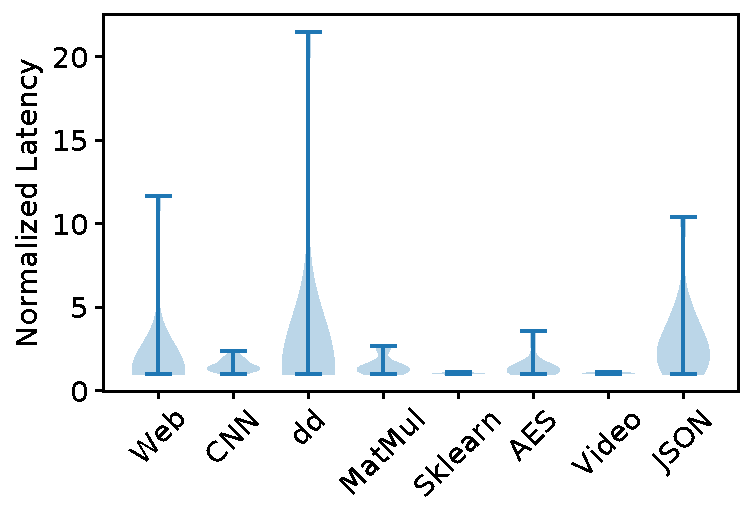
\includegraphics[width=0.33\textwidth]{../figs/ow/function_breakdown_min.pdf}
 % \vspace*{-0.25cm}
  \caption{Functions' warm latencies vary widely even under no system load, due to OpenWhisk jitter.}
  \label{fig:UnstableEmpty}
 %   \vspace*{-0.25cm}
  %XXX:Y Axis: Normalized latency
\end{figure}


% We also place the system under some load and examine how much of the end-to-end latency is spent in non-function computation.
% All functions, listed in Table~\ref{tab:overhead-times}, have a similar minimum overhead time of over one-hundreth of a second.
% While this is a significant time, the median times are all an order of magnitude higher.
% Fully half of function invocaitons spend a tenth of a second -often much more- stuck in the OpenWhisk pipeline.
% The baseline overhead time comes from the composite services of OpenWhisk communicating to invoke each function.
% Some of the more severe times we examined had the invoker waiting several seconds trying to inform the controller of a completed execution.
% The significant jitter encourages the use of a stale-load aware load balancing policy that is agnostic to such jitter.
% These forms of jitter mean that we cannot have an ``optimal'' load balancing policy from a latency perspective, as too many external variable affect a function's end-to-end latency.


\noindent \textbf{Load-sensitivity.} 
Furthermore, we have found that \emph{different functions are affected by server load differently.}
%
Figure~\ref{fig:LatencyVsLoad} shows the correlation between function latency and the Linux load-average of the server for different function types. 
The load-average is normalized to the number of CPU cores: thus a load-average of 2 in the figure for the 16-CPU VMs corresponds to a Linux load-average of 32.
The load on the servers was increased by increasing the number of concurrently executing functions of the same type.


We see that in general, as the server load increases, so does the latency of the function invocations.
Each point in the scatter-plots of Figure~\ref{fig:LatencyVsLoad} represents a unique invocation, with the latencies normalized to the lowest execution latency observed for that function.

The AES encryption function (Figure~\ref{fig:AES}) shows a gradual increase in latency as the load increases.
Surprisingly, the effect of load is minimal: the latency increases by ``only'' 2x even at a 10x load. 
%Nevertheless, does get affected by load, but surprisingly only under extreme cases where load is over 5!
The longer-running ML training function (Figure~\ref{fig:TRAIN}) also sees a correlation between server load and its end-to-end latency.
However, it's latency variance is lower because the longer running time (50 seconds) hides the variable OpenWhisk overhead.
Both functions presented here have the highest correlation between system load and latency, yet themselves do not have a high correlation.
Thus scheduling on an overloaded server can degrade function performance, it must be weighed against the performance penalty of a cold start.
% We describe this OpenWhisk ``system overhead'' more in Section~\ref{sec:unstable-latency}.
% Thus, running warm functions on overloaded functions comes with performance degradation risk, which is highly variable and hard to model, which presents yet another load-balancing challenge. 

%Note that while it's worst-case latency was 1.6 times the ideal, that represents an additional \emph{30 seconds} until it completes.
% \textbf{Alex: Earlier text said TRAIN had high correlation. But it doesnt (axes are not the same). It only shows less variance.}
%Certain functions see essentially no impact from server load, such as the web-server in Figure~\ref{fig:CHAM}, because they do not use much CPU or have extended runtimes.


\begin{figure}
  %\subfloat[]{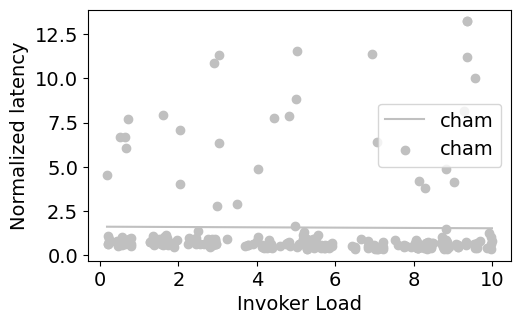
\includegraphics[width=0.22\textwidth]{../figs/lat-under-load/filtered/latency_to_load-loadAvg-cham.png} \label{fig:CHAM}}
  \subfloat{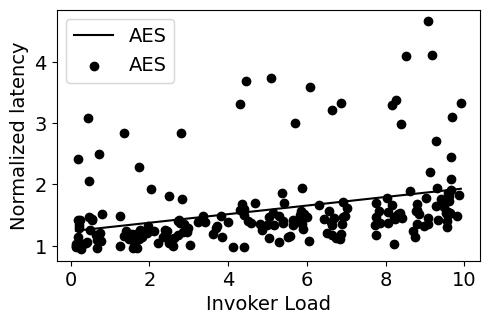
\includegraphics[width=0.22\textwidth]{../figs/lat-under-load/filtered/latency_to_load-loadAvg-aes.png} \label{fig:AES}}
  \subfloat{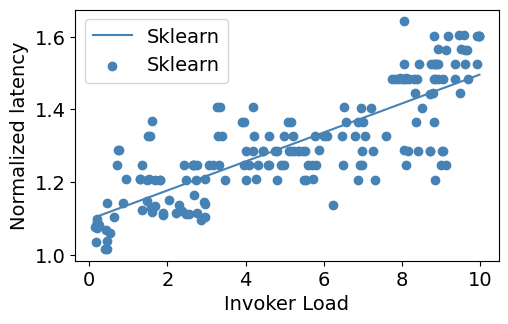
\includegraphics[width=0.22\textwidth]{../figs/lat-under-load/filtered/latency_to_load-loadAvg-train.png} \label{fig:TRAIN}}
%    \vspace*{-0.25cm}
  \caption{Latency increases due to system load, but is function-dependent.}
  \label{fig:LatencyVsLoad}
%  \vspace*{-0.25cm}
\end{figure}


% CH with bounded loads is a good idea, but 
% In a large cluster, cant assume perfect load information, which is especially challenging for
% Stale loads (Dahlin) and follow-up work: homogenenous requests making it easy to predict what the server load is going to be based on the number of requests sent. But not applicable here. 




%%% Local Variables:
%%% mode: latex
%%% TeX-master: "paper"
%%% End:
